\documentclass[letterpaper,10pt]{article}

\usepackage{titling}
\usepackage{listings}
\usepackage{url}
\usepackage{setspace}
\usepackage{subfig}
\usepackage{sectsty}
\usepackage{pdfpages}
\usepackage{colortbl}
\usepackage{multirow}
\usepackage{relsize}
\usepackage{amsmath}
\usepackage{fancyvrb}
\usepackage{amsmath,amssymb,amsthm,graphicx,xspace}
\usepackage[titlenotnumbered,noend,noline]{algorithm2e}
\usepackage[compact]{titlesec}
\usepackage[default]{droidserif}
\usepackage[T1]{fontenc}
\usepackage{tikz}
\usetikzlibrary{arrows,automata,shapes,trees,matrix,chains,scopes,positioning,calc}
\tikzstyle{block} = [rectangle, draw, fill=blue!20, 
    text width=2.5em, text centered, rounded corners, minimum height=2em]
\tikzstyle{bw} = [rectangle, draw, fill=blue!20, 
    text width=4em, text centered, rounded corners, minimum height=2em]

\definecolor{namerow}{cmyk}{.40,.40,.40,.40}
\definecolor{namecol}{cmyk}{.40,.40,.40,.40}

\let\LaTeXtitle\title
\renewcommand{\title}[1]{\LaTeXtitle{\textsf{#1}}}


\newcommand{\handout}[5]{
  \noindent
  \begin{center}
  \framebox{
    \vbox{
      \hbox to 5.78in { {\bf ECE155: Engineering Design with Embedded Systems } \hfill #2 }
      \vspace{4mm}
      \hbox to 5.78in { {\Large \hfill #4  \hfill} }
      \vspace{2mm}
      \hbox to 5.78in { {\em #3 \hfill} }
    }
  }
  \end{center}
  \vspace*{4mm}
}

\newcommand{\lecture}[3]{\handout{#1}{#2}{#3}{Lecture #1}}
\newcommand{\tuple}[1]{\ensuremath{\left\langle #1 \right\rangle}\xspace}

\addtolength{\oddsidemargin}{-1.000in}
\addtolength{\evensidemargin}{-0.500in}
\addtolength{\textwidth}{2.0in}
\addtolength{\topmargin}{-1.000in}
\addtolength{\textheight}{1.75in}
\addtolength{\parskip}{\baselineskip}
\setlength{\parindent}{0in}
\renewcommand{\baselinestretch}{1.5}
\newcommand{\term}{Spring 2014}

\singlespace


\begin{document}

\lecture{ 28 --- Simulation}{\term}{Patrick Lam \& Jeff Zarnett}

Here are a bunch of simulations:

\begin{tabular}{ll}
\url{http://www.youtube.com/watch?v=HUGjUvjtwS8} & physics N-body simulation \\
\url{http://www.youtube.com/watch?v=JGyJqXJWkuY} & aircraft \\
\url{http://www.youtube.com/watch?v=No5N6uYJaNk} & nuclear plant control room\\
\url{https://www.youtube.com/watch?v=bRgFuwG4nYg} & Kerbal Space Program
\end{tabular}

\paragraph{Basic Idea.} Create a model of a system to investigate 
its behaviour.

A \emph{simulation} evaluates a mathematical model of a system to
estimate the behaviour of the system.

These days, most simulations use computers to evaluate the state of
the system. However, you could think of some board games as a
primitive sort of simulation.

\subsection*{Why Simulate?}
Building the system and testing on it always gives more accurate
results. However, testing on the actual system is sometimes impossible:
\begin{itemize}
\item the system may not exist yet (e.g. proposed commercial jet design);
\item the system may be costly to use (e.g. space shuttle);
\item the system may be dangerous to use (e.g. nuclear reactor);
\item the system may be disrupted by use (e.g. animal migration); or
\item you just don't have enough access to the system (e.g. phones).
\end{itemize}

The next best thing, then, is to simulate. You might be forced to
simulate when experimenting with an actual system is infeasible, too
costly, too dangerous, or too disruptive to the system. Or you can simulate
for fun and profit (e.g., a computer game).

\subsection*{Models are Inherently Wrong}
\begin{quote}
\textit{...essentially, all models are wrong, but some are useful.}
\end{quote}
\hfill George E. P. Box

It's important to remember that a simulation is an abstraction of the real world and it does not actually contain all the details of reality. This is frequently necessary because reality is too complex or expensive to model. A physics model might ignore the effects of friction between small objects. This is, in the strictest sense, incorrect, but at some point we decide the error is small enough that we can ignore it. For example, $\pi$ has an infinite number of digits, but after the first thousand digits or so, the error introduced by rounding the value off is so small it has no relevance for architectural calculations. It is not as accurate as it could be, but it is ``good enough''. Deciding when we are at the point of ``good enough'' is a matter of engineering judgement.

Models usually have a range of validity which must be respected if the model is to be useful. This is something you have probably seen in physics. Newton's equations are valid as a model for motions of bodies as long as the bodies are not moving at relativistic speeds (and in general if the speed is below 0.1$c$, where $c$ is the speed of light in vacuum, the error is so small it can be ignored). If you try to apply Newton's model outside of its range of validity, such as at speeds of 0.5$c$, your answer will be incorrect. Instead, you should apply Einstein's relativistic equations; a different model, which has a different range of validity. When using or creating a model, it is definitely important to understand its limitations.

\begin{quote}
\textit{The map is not the territory.}
\end{quote}
\hfill Alfred Korzybski

Do not confuse the map (an abstract representation of reality) with the territory (reality). Studying the model and the output of the model can be helpful, but it is only a tool to aid understanding of reality. It is possible to invest too much time into simulation or building the simulation, and not enough time in understanding the challenges of the real world. At some point, you will have to build or use the real thing. 

A rather literal example of how the map is not the territory: the Canada-US Border, west of the province of Ontario, is drawn on most maps as being exactly the $49^{th}$ parallel. This is, however, wrong. When the border was officially marked, the surveyors did so by placing small monuments at discrete distances. The border is legally the series of line segments connecting these monuments. Given the level of technology available at the time of measurement, these are not in a perfectly straight line. And even a map representing those is wrong. Even if there are no significant drawing errors, shrinking the scale from thousands of kilometres of country down to a map measured in centimetres will introduce error and inaccuracy: the point marking the placement of the monument might be the finest resolution the printer can print and still represent an area over 100m in diameter - where exactly in the 100m-diameter circle is the monument?


\subsection*{Case Studies}
We will discuss two case studies, both related to the robots that
students programmed in previous offerings of this class. The case
studies simulate the robots with varying degrees of accuracy.

\paragraph{Coarse Simulation.} Here's one design for a Lego robot and
environment simulator: 

\begin{itemize}
\item Create a class {\tt Board}. Other classes can query this 
class to find out whether the board is black or white
at a certain point.
\item Create a class {\tt Robot}. This class stores, in fields, the
  current position and velocity of the robot, and contains the main
  logic of the robot.
\item Create a class {\tt LightSensor}. The {\tt Robot} gets light
readings from the {\tt LightSensor} which are appropriate to its
position on the {\tt Board}.
\end{itemize}

Then you can have a main simulation driver which calls the {\tt Robot}
to (1) update its position according to the velocity; and (2) turn the
robot if necessary. (You would probably program these actions in
different methods.) Note that each call to the {\tt Robot} would
simulate the effect of time moving forward by one time-step.

\paragraph{Detailed Simulation: Visual Simulation Environment.}
It is possible to simulate the same system at many different levels of
detail. For instance, Microsoft's Visual Simulation Environment
simulates the behaviour of your robot code much more realistically.

In particular, VSE creates a simulated world and evaluates the 
behaviour of physical objects within that simulated world.
This simulation resembles step (1) in the coarse-grained simulation,
except that it tracks the behaviour of multiple objects and has a
more-detailed model of the environment than just a {\tt Board}.

VSE also calls your actual code to simulate the behaviour
of your control software. This is like step (2) in the coarse-grained
simulation, but in this case it is running actual code.

\paragraph{Caveat.} Simulations aren't perfect. 
For instance, a previous lab report reported that everything worked
fine in simulation under VSE, but needed lots more work to work on the
actual robot.

{\sf Why?}\\[2em]


The Android emulator is pretty good as far as it goes, but it's
difficult for it to emulate accelerometer readings.

\subsection*{Other Examples} 
You might simulate a digital logic circuit using discrete techniques,
since gates change values at specific times, in response to changing
inputs.

On the other hand, you might simulate an analog circuit using continuous
techniques, since the voltages and currents change continuously with
respect to time.

In terms of writing a simulation, you would use different techniques
to implement discrete simulations (queue-based: put the time of next
event into the queue) and continuous simulations (numerically
integrate an ordinary differential equation over and over; see
ECE204).




\paragraph{Classifying Simulations.}
Here are three orthogonal axes along which you can classify simulations.

Continuous vs. Discrete Simulation Models:
\begin{itemize}
\item A \emph{continuous} simulation model represents a system with continuously changing state variables.
\item A \emph{discrete} simulation model represents a system with discrete state changes.
\end{itemize}

\begin{center}
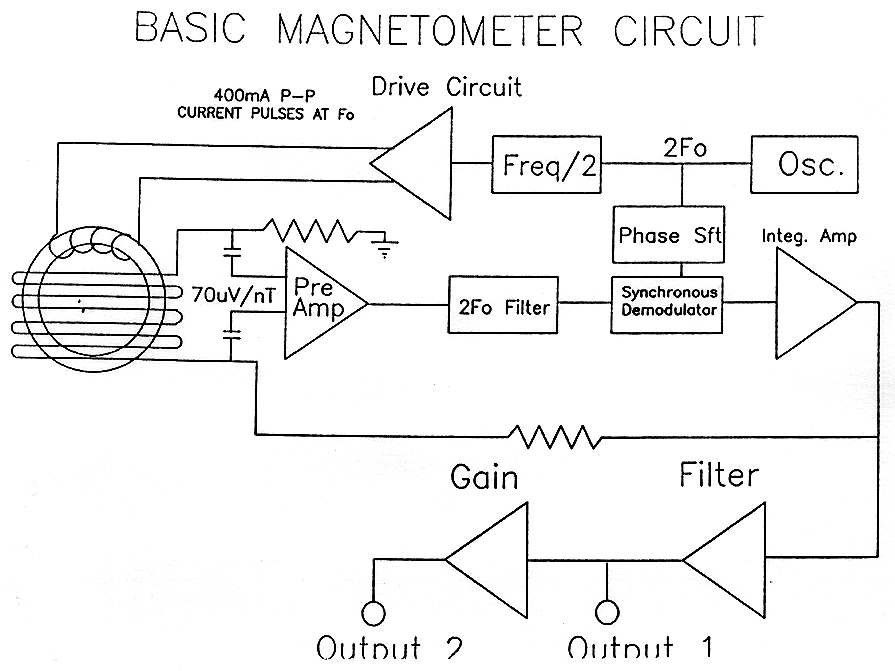
\includegraphics[width=.7\textwidth]{images/fig6}~\cite{magneto}
\end{center}

Dynamic vs. Static Simulation Models: 
\begin{itemize}
\item A \emph{dynamic} simulation model represents a system as it evolves over time; it recomputes the state of the system at various times.
\item A \emph{static} simulation model is a one-shot deal: you feed it some conditions and it tells you the result. This is useful for what-if simulations: if I price my cookies at \$2, how many will I sell?
\end{itemize}

Deterministic vs. Stochastic Simulation Models:
\begin{itemize}
\item A \emph{deterministic} simulation model exactly computes the simulated state of the system at every step (subject to inaccuracies in the calculations).
\item A \emph{stochastic} simulation model uses randomness to (accurately!) estimate the expected behaviour of the system without computing the behaviour of each particle; it relies on the underlying randomness of the system components.
\end{itemize}
% bring in some chocolates or something and stochastically throw them
% at the students

\paragraph{Simulation Tools.} While you'd have to develop your own tools
in certain domains, others domains have well-supported tools. These
tools allow you to rapidly prototype a simulation of a complex system
and its environment. However, you must understand how the tool works
before relying on it. Here are some examples:

\begin{itemize}
\item \emph{Microsoft Visual Simulation Environment} simulates decentralized software services for robots.
\item \emph{Arena} simulates businesses, services, and manufacturing processes.
\item \emph{Simulink} simulates a variety of time-varying systems, including communications, controls, signal processing, video processing, and image processing; people use it to investigate and verify implementations of these systems.
\item \emph{SPICE} and its many variants can be used to simulate analog circuits.
\end{itemize}

General-purpose simulation languages also exist to aid in the
development of complex, application-specific simulation tools.

\bibliographystyle{alpha}
\bibliography{155}


\end{document}
